\section{Time-Dependent Perturbation Theory}
Let us review what we did last class (and not just the formula, but when the formula applies!) We had the Hamiltonian:
\begin{equation}
    H = H^0 + H'(t).
\end{equation}
In QM up until this point, the eigenstates $H^0$ were totally stable/stationary in time. But of course in nature this is not what happens; we have transitions of states. This is why we start to think about time-dependent Hamiltonians. We derived:
\begin{equation}
    \begin{split}
        \dot{c}_a &= -\frac{i}{\hbar}c_b \bra{\psi_a}H'\ket{\psi_b}e^{-i\omega t}
        \\ \dot{c}_b &= -\frac{i}{\hbar}c_a \bra{\psi_b}H'\ket{\psi_a}e^{i\omega t}
    \end{split}
\end{equation}
with:
\begin{equation}
    \omega = \frac{E_b - E_a}{\hbar}.
\end{equation}
The only simplification that went into this was $\bra{\psi_a}H'\ket{\psi_b} = 0$ (but this is harmless and we could do without it). Up until this point, we have made no assumptions. But let us enforce some now.

\subsection{First-Order Time-Dependent Perturbation Theory}
Let us assume $c_a(t = 0) = 1$ and $c_b(t = 0) = 0$ (though we can make an arbitrary choice of initial conditions). Now, we make an assumption that $c_b = 0$ and $c_a = 1$ in the above formula (i.e. in the above formulas we assume that the $c_b/c_a$ on the RHS are \emph{not} time dependent). We can then proceed to discuss corrections to this formula, but this involves higher orders of perturbation theory. The only differential equation we need to solve under this approximation is:
\begin{equation}
    \dot{c}_b = -\frac{i}{\hbar}\bra{\psi_b}H'(t)\ket{\psi_a}e^{i\omega t}
\end{equation}
Which has solution:
\begin{equation}
    c_b(t) = -\frac{i}{\hbar}\int_0^t dt' e^{i\omega t'}\bra{\psi_b}H'(t')\ket{\psi_a}
\end{equation}
The probability to find the state in the $b$ state is then nothing but:
\begin{equation}
    P_b(t) = \frac{1}{\hbar^2}\left|\int_0^t dt' e^{i\omega t'}\bra{\psi_b}H'(t')\ket{\psi_a}\right|^2
\end{equation}

\subsection{Second-Order Time-Dependent Perturbation Theory}
To second order, we consider plugging our first-order solution for $c_b(t)$ back into the $c_a(t)$ equation, so:
\begin{equation}
    \dod{c_a}{t} = -\frac{i}{\hbar}\bra{\psi_a}H'(t)\ket{\psi_b}e^{-i\omega t}\left(-\frac{i}{\hbar}\right)\int_0^t dt' e^{i\omega t'}\bra{\psi_b}H'(t')\ket{\psi_a}
\end{equation}
and so:
\begin{equation}
    c_a(t) = -\frac{1}{\hbar^2}\int_0^t dt' e^{-i\omega t'}\bra{\psi_a}H'(t')\ket{\psi_b}\int_0^{t'}dt'' e^{i\omega t''}\bra{\psi_b}H'(t'')\ket{\psi_a}
\end{equation}
The third order perturbation theory (and higher orders) follow by continuing to iterate as we have done above (solve for the coefficients at a lower order, then plug them back into the differential equation and solve). Formally, the full perturbative expansion can be written down as a Dyson series. But often the lower order terms are sufficient to probe interesting physical effects.

\subsection{Example: Exponentially Decaying Electric Field Pulse}
We consider a electric field with temporal profile:
\begin{equation}
    E(t) = E_0e^{-t^2/\tau^2}
\end{equation}
so our perturbing Hamiltonian is:
\begin{equation}
    H'(t) = -eE_0e^{-t^2/\tau^2}z
\end{equation}

\begin{figure}[htbp]
    \centering
    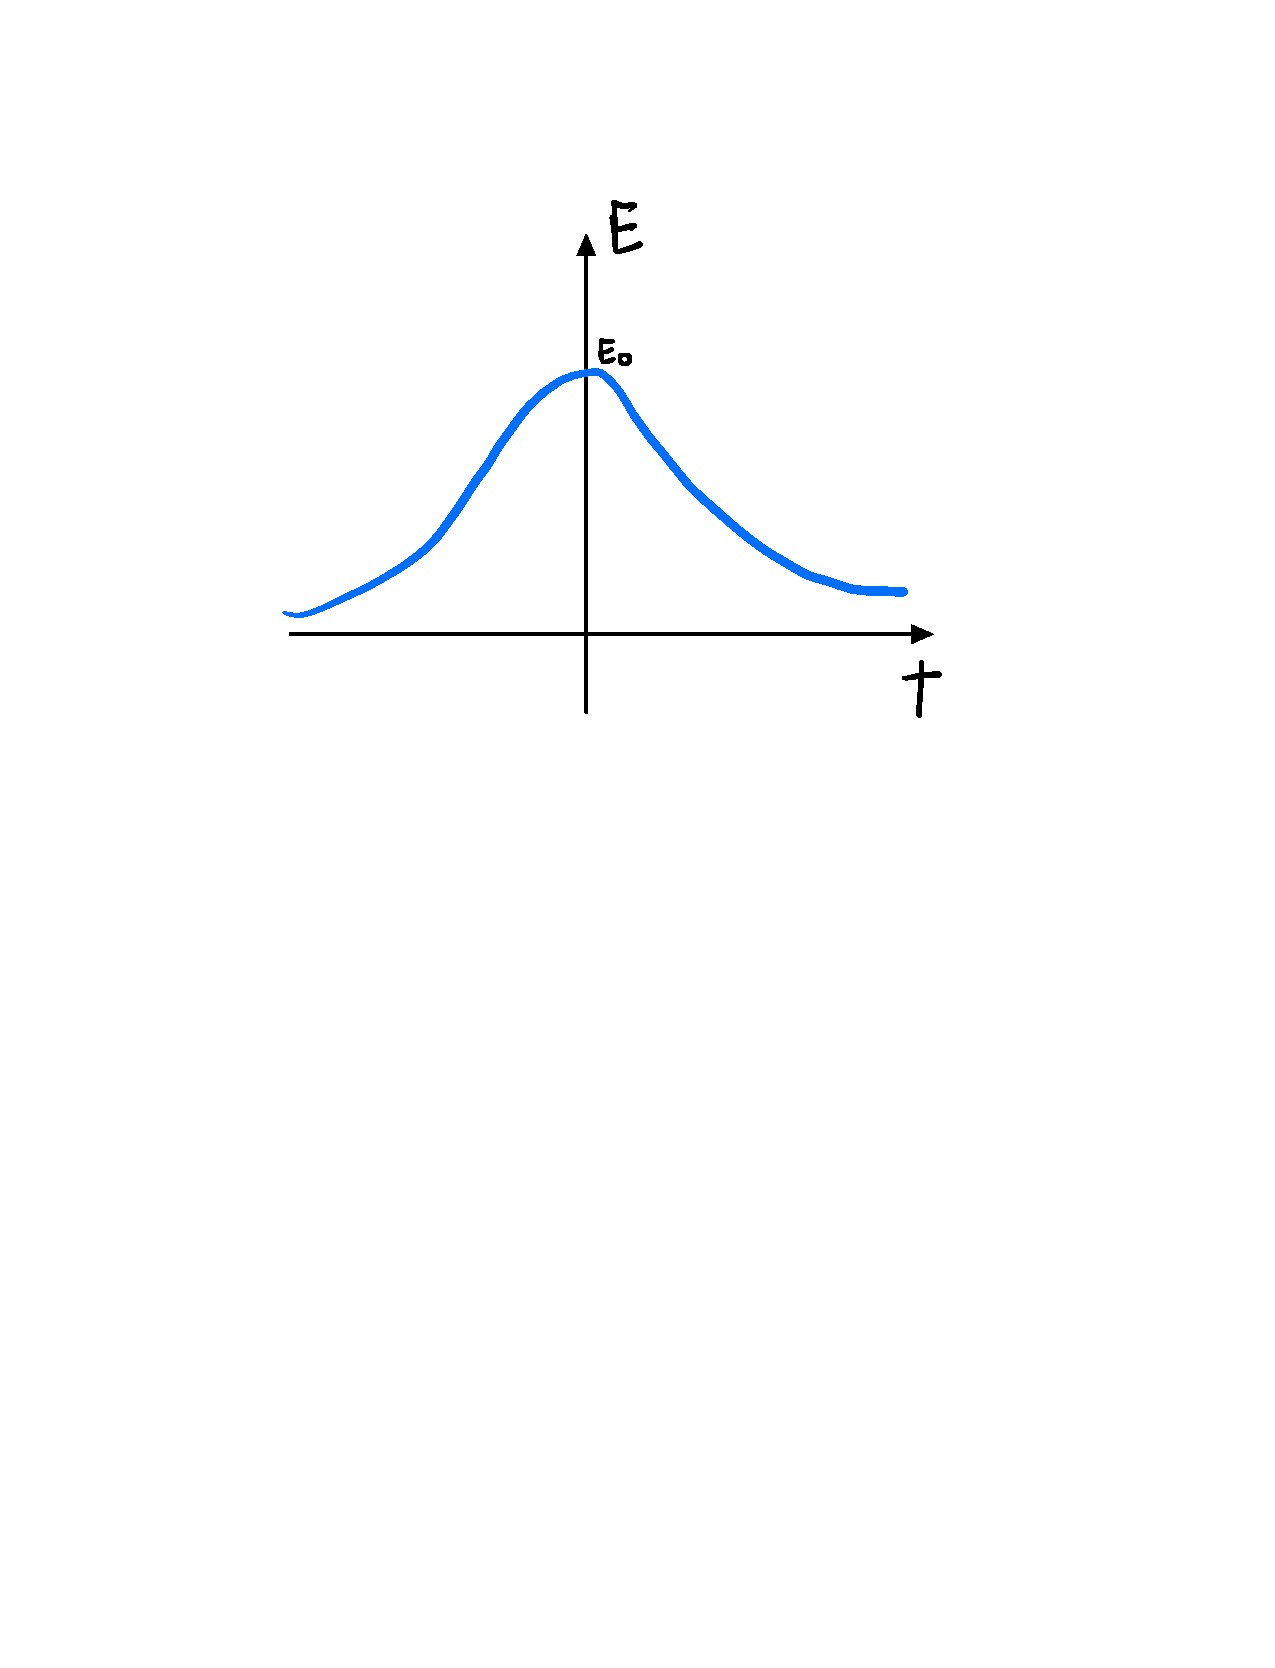
\includegraphics[scale=0.6]{Images/fig-gaussianpulse.pdf}
    \caption{Sketch of the gaussian pulse of the electric field.}
    \label{fig-gaussianpulse}
\end{figure}

We suppose that our state starts in the $\ket{100}$ state. We want to determine the transition probability to $\ket{n \neq 0, l = 1, m = 0}$ We recall from our selection rules that:
\begin{equation}
    \bra{nlm}z\ket{100} \neq 0
\end{equation}
in the case where $l = 1$ (different parity) and $m = 0$ (same magnetic quantum number). Using our first-order perturbation theory result. then find the transition coefficient of:
\begin{equation}
    c_b(t = \infty) = -\frac{i}{\hbar} \int_{-\infty}^\infty dt' e^{i\omega t'} e^{-t'^2/\tau^2}\left(-eE_0\avg{z}\right)
\end{equation}
Where $\avg{z} \sim a_B$. To compute the integral in the above, we complete the square:
\begin{equation}
    \int_{-\infty}^\infty dt' e^{i\omega t'} e^{-t'^2/\tau^2} = \int_{-\infty}^\infty dt' e^{\frac{1}{-\tau^2}\left(t' - \frac{i\tau^2\omega}{2}\right)^2}e^{\frac{1}{\tau^2}\left(\frac{i\tau^2\omega}{2}\right)^2} = \sqrt{\pi \tau^2}e^{-\frac{\tau^2\omega^2}{4}}
\end{equation}
where we have evaluated the integral by considering that it is nothing but the famous Gaussian. And so we find:
\begin{equation}
    \abs{c_b}^2 = \frac{\pi\tau^2}{\hbar^2}e^{-\frac{\tau^2\omega^2}{2}}\abs{\bra{nlm}z\ket{100}}^2
\end{equation}
The latter coefficient we can say is $a_B^2$ by dimensional consideration; we don't care that much about it:
\begin{equation}
    \abs{c_b}^2 = \frac{\pi\tau^2a_B^2}{\hbar^2}e^{-\frac{\tau^2\omega^2}{2}}
\end{equation}
Note that all of this was justified if:
\begin{equation}
    \abs{c_b}^2 \ll 1
\end{equation}
There are two cases of interest:
\begin{enumerate}
    \item $\omega \tau \gg 1$; i.e. the adiabatic approximation, where the external field changes very slowly. In this limit, this has no chance of actually causing a transition. We can see this from the formula but also physical intuition; the quickly changing degrees of freedom of the systems change must faster than the perturbation. As an example, atoms don't care about the (comparitively much slower) expansion of the universe! In this case, we have:
    \begin{equation}
        P_{a \to b}(t = \infty) \sim e^{-\tau^2\omega^2} \ll 1
    \end{equation}
    \item $\omega \tau \ll 1$; i.e. an instantaneous perturbation/a very short pulse. In this case, we have that the exponential term can be neglected (it is close to one) and so:
    \begin{equation}
        P_{a \to b} \sim \abs{\pi \tau^2 e^2 E_0^2 a^2}{\hbar^2} \ll 1
    \end{equation}
    And from the $\omega \tau \ll 1$ condition we can write:
    \begin{equation}
        P_{a \to b} \sim \abs{\pi \tau^2 e^2 E_0^2 a^2}{\hbar^2} \ll \frac{\pi e^2E_0^2 a^2}{\hbar^2\omega^2} = \frac{\pi e^2E_0^2 a^2}{(E_a - E_b)^2}
    \end{equation}
    where in the last equality we invoke the definition of $\omega$. Let's look at the physical meaning of this last expression:
    \begin{equation}
        \frac{\abs{eE_0a}}{E_a - E_b} \ll 1
    \end{equation}
    and so:
    \begin{equation}
        E_0 \ll \frac{10\si{eV}}{e 10^{-8}\si{cm}} = 10^9 \si{V.cm^{-1}}
    \end{equation}
    which is justified. We also note that the transition is most likely when the pulse timescale is on the same order as the frequency timescale (might have got this wrong - didn't quite follow).
\end{enumerate}

We will not discuss instantaneous perturbation theory much further. Usually, the way it is treated that you have one Hamiltonian and then at some time you turn on a new Hamiltonian suddenly. The system then does not have time to adjust to the new Hamiltonian, so you can expand the old state in terms of the new ones etc... There are many physical examples (e.g. $\beta$-decay). 

We will however explore the adiabatic approximation much further. There are many interesting implications here for condensed matter such as Berry phase, topological phases etc.

Next class, we discuss perturbation theory for the case when we have a periodic potential. After this, we discuss how to compute transitions.